\chapter{Hidup Tumbuhan: Berjaya sambil Berakar}\label{ch:g12:plant-rooted-life}

Sebatang pohon ek tak dapat berjalan menuju air, lari dari seekor ulat,
atau pergi mencari pasangan. Ia berdiri di tempat bijinya jatuh selama
tiga abad, dan dalam kurun itu ia mengangkat ratusan ton air dari
tanah, menangkis ribuan \omterm{def:g10:biodiversity-scales:species}{spesies} yang hendak memakannya, memutar daunnya
mengikuti cahaya, dan mengirimkan serbuk sari serta bijinya ke seluruh
pedesaan lewat angin dan lewat burung jay. Hidup berakar bukanlah hidup
yang pasif; ia adalah seperangkat pemecahan yang berbeda bagi masalah
yang sama --- makan, membela diri, berpindah, berbiak --- dan bab ini
meninjaunya satu per satu.

\section{Tubuh yang dibangun untuk pertukaran}

\begin{proposition}[Dua sistem, dua permukaan]\label{prop:g12:plant-rooted-life:surfaces}
Tumbuhan berbunga tersusun dalam dua sistem: \emph{sistem akar} di
dalam tanah, yang menyerap air dan ion mineral serta melabuhkan
tumbuhannya, dan \emph{sistem tajuk} di udara --- batang dan daun ---
yang menangkap cahaya dan karbon dioksida. Masing-masing adalah
permukaan pertukaran yang luas: daun sebatang pohon besar membentangkan
beberapa ratus meter persegi permukaan ke arah cahaya, dan akarnya,
yang diperpanjang oleh miliaran \emph{rambut akar}\index{rambut akar}
mikroskopis, beberapa ratus meter persegi ke arah tanah. Tumbuhan,
di atas segalanya, adalah cara membentangkan permukaan ke dua arah
dari satu titik tetap.
\end{proposition}
\begin{proof}[Bukti percobaan]
Sebatang gandum hitam yang ditanam empat bulan dalam sekotak tanah
ternyata punya $\num{1.4e10}$ \omterm{prop:g12:plant-rooted-life:surfaces}{rambut akar} dengan panjang seluruhnya
lebih dari \qty{10000}{km} dan luas permukaan sekitar \qty{400}{m^2},
sepuluh kali luas daunnya. Sebatang pohon ek dewasa membawa sekitar
250\,000 helai daun; satu hektar hutan menyodorkan
\qtyrange{5}{8}{ha} permukaan daun ke langit. Memotong \omterm{prop:g12:plant-rooted-life:surfaces}{rambut akar}
sebuah semai, atau melapisi daunnya, menghentikan pertumbuhannya dalam
hitungan hari.
\end{proof}

\begin{omfigure}
\begin{tikzpicture}
  \node[anchor=south west, inner sep=0] (img) at (0,0)
    {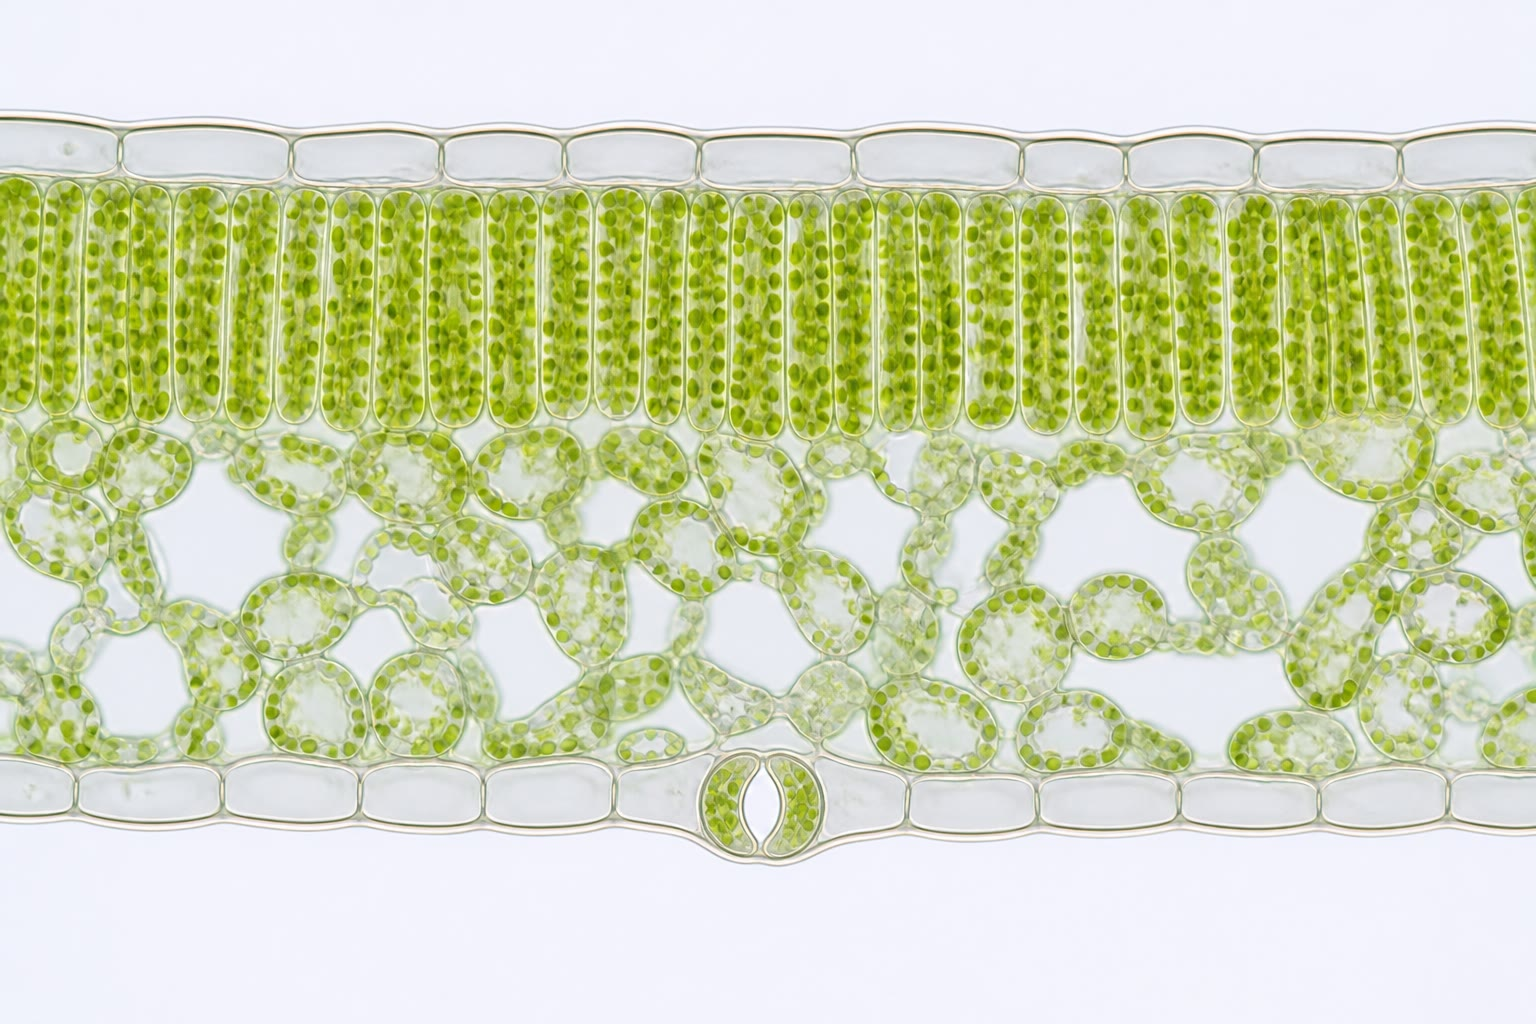
\includegraphics[width=0.56\linewidth]{images/book2/ai/fig-leaf-cross-section.jpg}};
  \begin{scope}[x={(img.south east)}, y={(img.north west)},
      every node/.style={font=\small}]
    \draw[omDef, thick] (0.50,0.88) -- (0.50,1.08) node[above] {kutikula dan epidermis atas};
    \draw[omDef, thick] (0.20,0.72) -- (-0.04,0.85) node[left, align=right] {sel palisade,\\ penuh kloroplas};
    \draw[omDef, thick] (0.20,0.42) -- (-0.04,0.30) node[left, align=right] {lapisan bunga karang\\ berongga udara};
    \draw[omDef, thick] (0.50,0.20) -- (0.50,-0.06) node[below] {stoma di antara dua sel penjaga (epidermis bawah)};
    \draw[omDef, thick] (0.85,0.12) -- (1.04,0.05) node[right] {epidermis bawah};
  \end{scope}
\end{tikzpicture}

{\small Sehelai daun dalam irisan. Cahaya masuk lewat kulit atas yang
bening menuju \omterm{def:g10:cells-common-unit:cell}{sel} palisade, yang padat oleh \omterm{def:g10:cells-common-unit:organelle}{kloroplas}; karbon dioksida
masuk lewat stomata kulit bawah dan berdifusi melalui rongga udara
lapisan bunga karang menuju \omterm{def:g10:cells-common-unit:cell}{sel} yang memakainya.}
\end{omfigure}

\begin{definition}[Stomata]\label{def:g12:plant-rooted-life:stomata}
Sebuah \emph{stoma}\index{stoma} adalah liang pada kulit daun, yang
dibatasi dua \emph{\omterm{def:g10:cells-common-unit:cell}{sel} penjaga} yang membukanya dengan menggembung dan
menutupnya dengan mengempis. Lewat stoma yang terbuka, karbon dioksida
masuk untuk \omterm{def:g10:cell-metabolism:autotrophy}{fotosintesis} dan uap air keluar --- \emph{transpirasi}
yang tak dapat dihindari tumbuhan selama ia makan. Sehelai daun
membawa seratus sampai tiga ratus stoma per milimeter persegi,
terutama di permukaan bawahnya; stoma membuka dalam cahaya dan menutup
dalam gelap serta dalam kekeringan.
\end{definition}

\begin{omfigure}
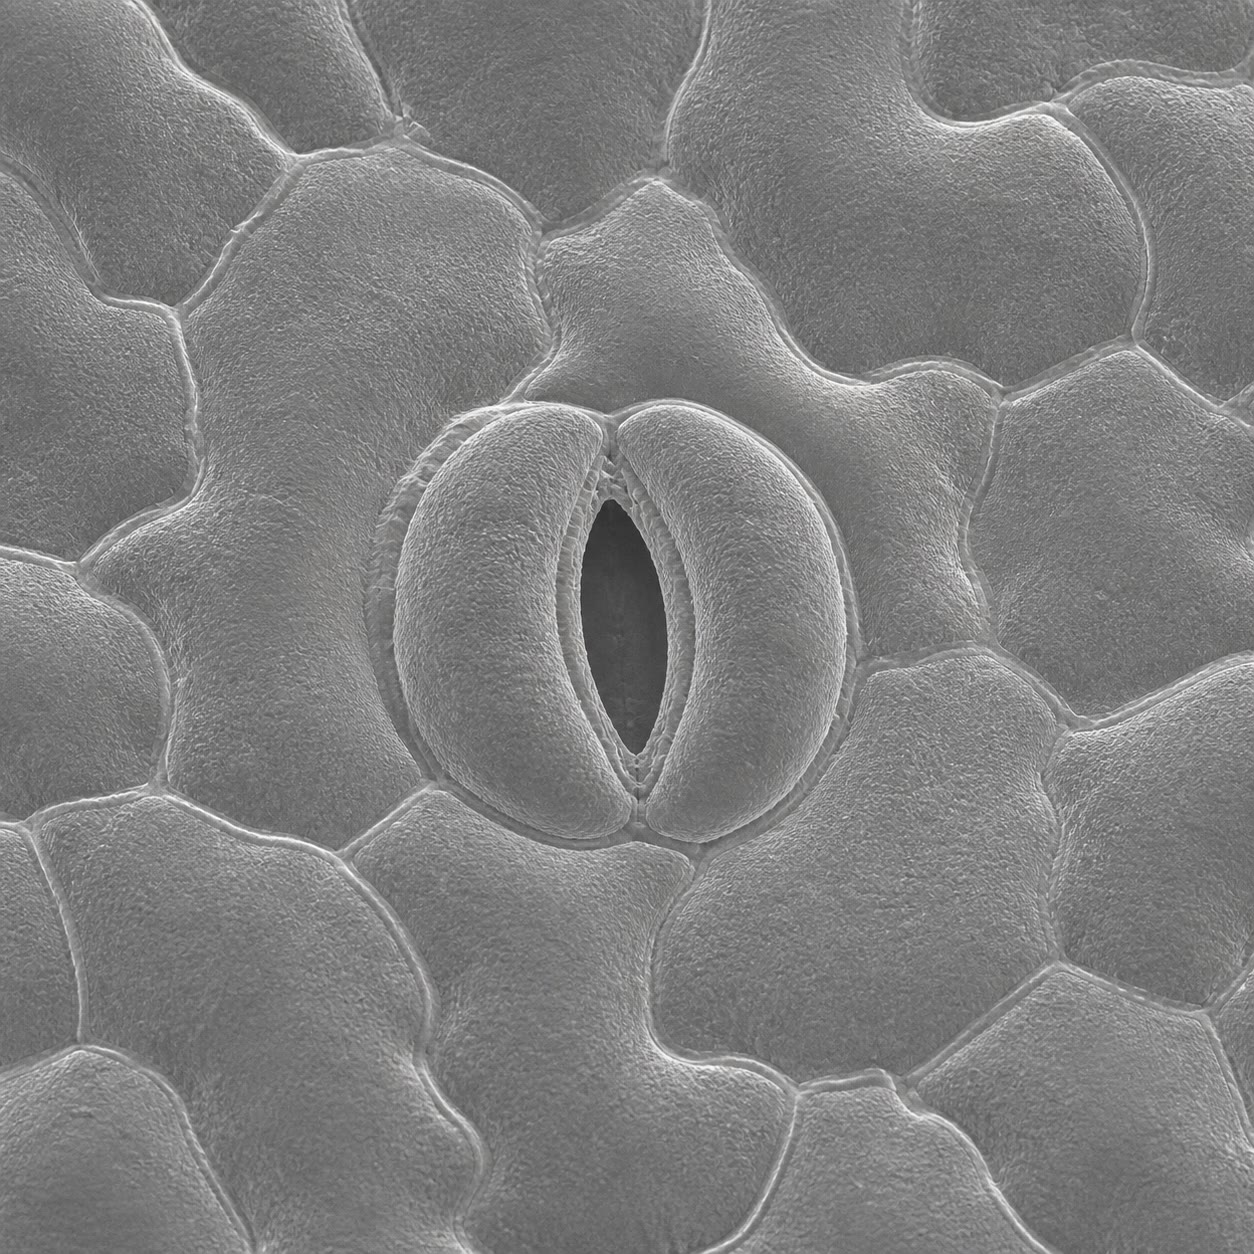
\includegraphics[width=0.4\linewidth]{images/book2/ai/g12-plant-stoma-sem.jpg}

{\small Sebuah \omterm{def:g12:plant-rooted-life:stomata}{stoma} dilihat dengan mikroskop elektron payar: kedua
\omterm{def:g10:cells-common-unit:cell}{sel} penjaga berbentuk ginjal mengelilingi liangnya, di antara \omterm{def:g10:cells-common-unit:cell}{sel}
pipih kulit daun. Liangnya selebar beberapa mikrometer.}
\end{omfigure}

\begin{omfigure}
\begin{tikzpicture}
\begin{axis}[
  width=0.86\linewidth, height=5.4cm,
  axis x line=bottom, axis y line=left,
  xmin=0, xmax=24, ymin=0, ymax=110,
  xlabel={jam dalam sehari}, ylabel={\% dari maksimum},
  xlabel style={font=\small, at={(axis description cs:0.5,-0.12)}, anchor=north},
  ylabel style={font=\small},
  tick label style={font=\small}, xtick={0,6,12,18,24}, ytick={0,50,100},
  legend style={at={(0.5,-0.3)}, anchor=north, legend columns=3, font=\small, draw=none},
]
\addplot[thick, omProp, smooth] coordinates {(0,0) (5,0) (6,20) (8,80) (12,100) (16,80) (19,20) (20,0) (24,0)};
\addplot[thick, omMeth, smooth] coordinates {(0,5) (5,5) (7,60) (9,95) (13,90) (15,40) (17,70) (19,30) (20,5) (24,5)};
\addplot[thick, omDef, dashed, smooth] coordinates {(0,3) (5,3) (7,50) (9,85) (13,100) (15,45) (17,65) (19,25) (20,3) (24,3)};
\legend{cahaya, bukaan stoma, transpirasi}
\end{axis}
\end{tikzpicture}

{\small Sehari musim panas bagi sehelai daun. \omterm{def:g12:plant-rooted-life:stomata}{Stomanya} membuka bersama
cahaya dan menutup pada malam hari; pada sore yang panas \omterm{def:g12:plant-rooted-life:stomata}{stoma} menutup
sebagian untuk membatasi kehilangan air, dan transpirasi --- yang
mengikuti bukaannya --- ikut melandai.}
\end{omfigure}

\section{Mengalirkan air dan makanan tanpa jantung}

\begin{proposition}[Dua getah]\label{prop:g12:plant-rooted-life:saps}
Tumbuhan punya dua sistem pengangkutan, keduanya tersusun dari \omterm{def:g10:cells-common-unit:cell}{sel}
panjang yang bersambung menjadi tabung di dalam urat setiap organnya.
\begin{itemize}
  \item \emph{Xilem}\index{xilem} mengangkut \emph{getah mentah} ---
        air dan ion mineral yang diserap akar --- ke atas menuju
        daunnya. Gaya penggeraknya adalah transpirasi: air yang
        menguap dari \omterm{def:g10:cells-common-unit:cell}{sel} daun menarik kolom air yang malar di dalam
        \omterm{prop:g12:plant-rooted-life:saps}{xilem} naik dari akar, seperti sumbu menarik minyak. Tanpa
        pompa, tanpa energi yang dikeluarkan tumbuhannya: mataharilah
        yang mengangkat.
  \item \emph{Floem}\index{floem} mengangkut \emph{getah olahan} ---
        air berisi gula yang dibuat daun --- dari daun ke setiap organ
        yang memakainya atau menyimpannya: pucuk yang tumbuh, akar,
        buah, biji, umbi. Getah itu mengalir dari sumber ke lubuk, ke
        arah mana pun lubuknya berada.
\end{itemize}
\end{proposition}
\begin{proof}[Bukti percobaan]
Batang terpotong yang ditaruh dalam air berpewarna menunjukkan pewarna
naik di dalam \omterm{prop:g12:plant-rooted-life:saps}{xilem}, lebih cepat pada tunas yang bertranspirasi
daripada pada tunas yang terkurung dalam kantong; tunas yang daunnya
dibuang tak mengangkat apa pun. Sebentuk cincin kulit kayu (yang berisi
\omterm{prop:g12:plant-rooted-life:saps}{floem}) yang dilepas dari batang menghentikan gula mencapai akar,
sehingga akarnya kelaparan dalam beberapa bulan, sedangkan daun di atas
cincin itu tetap dipasok air; gula menumpuk di atas cincin dan kulit
kayunya membengkak. Kutu daun yang mengisap \omterm{prop:g12:plant-rooted-life:saps}{floem} dengan mulutnya yang
mirip jarum, bila dipisahkan dari jarumnya, meneteskan setetes getah
manis yang bertekanan.
\end{proof}

\begin{omfigure}
\begin{tikzpicture}[font=\small, >=Stealth, line cap=round]
  % plant: roots, stem, leaves, fruit
  \draw[line width=6pt, omProp!40] (0,0) -- (0,5.5);           % stem
  \draw[thick, fill=omMeth!40] (0,4.6) .. controls (-1.2,5.0) and (-1.6,4.0) .. (-0.2,3.9) -- cycle;   % left leaf
  \draw[thick, fill=omMeth!40] (0,3.4) .. controls (1.2,3.8) and (1.6,2.8) .. (0.2,2.7) -- cycle;      % right leaf
  \draw[thick, fill=omThm!40] (0.9,5.4) circle (0.35);                                                 % fruit
  \draw[thick, omProp!60] (0,5.5) -- (0.7,5.3);
  \foreach \a in {-150,-120,-90,-60,-30} \draw[thick, omProp!70] (0,0) -- (\a:1.8);                   % roots
  \node[anchor=north] at (0,-1.9) {akar: menyerap air dan mineral};
  % xylem arrow (up)
  \draw[->, very thick, omDef] (-0.4,-1.2) -- (-0.4,4.4);
  \node[omDef, anchor=east, align=right] at (-0.6,1.5) {getah mentah: air\\ dan mineral,\\ ditarik naik oleh\\ transpirasi};
  % phloem arrows (from leaves down and up)
  \draw[->, very thick, omThm] (0.4,3.0) -- (0.4,0.0) -- (0.4,-1.0);
  \draw[->, very thick, omThm] (0.4,3.6) -- (0.4,5.2) -- (0.75,5.2);
  \node[omThm, anchor=west, align=left] at (0.7,1.2) {getah olahan:\\ gula dari daun\\ ke akar, buah,\\ dan pucuk tumbuh};
  \draw[->, thick, gray] (-2.4,4.6) -- (-1.6,4.6) node[pos=0, left, align=right, font=\scriptsize] {uap air\\ meninggalkan daun};
  \draw[<-, thick, gray] (-1.7,4.2) -- (-2.5,4.2);
\end{tikzpicture}

{\small Kedua aliran itu. Getah mentah naik di dalam \omterm{prop:g12:plant-rooted-life:saps}{xilem} dari akar ke
daun, ditarik oleh air yang menguap lewat stomata; getah olahan
berjalan di dalam \omterm{prop:g12:plant-rooted-life:saps}{floem} dari daun ke mana pun gula dipakai atau
disimpan --- turun ke akar, naik ke sebutir buah.}
\end{omfigure}

\begin{example}[Angka sebatang pohon]\label{ex:g12:plant-rooted-life:numbers}
Sebatang pohon birch dewasa pada hari musim panas mentranspirasikan
\qtyrange{300}{400}{L} air, yang diangkat setinggi \qty{20}{m}
melalui tabung \omterm{prop:g12:plant-rooted-life:saps}{xilem} selebar sepersepuluh milimeter dengan laju
\qtyrange{1}{5}{m} per jam. Kurang dari 1\% air itu disimpan untuk
\omterm{def:g10:cell-metabolism:autotrophy}{fotosintesis}; sisanya adalah harga \omterm{def:g12:plant-rooted-life:stomata}{stoma} yang terbuka. Sebagai
imbalannya daun mengikat sekitar \qty{5}{kg} karbon dioksida menjadi
\qty{3.5}{kg} gula, dan sebagian darinya diantarkan \omterm{prop:g12:plant-rooted-life:saps}{floem} ke setiap
ujung akar dan setiap biji yang memasak.
\end{example}

\section{Bertahan di tempat sendiri}

\begin{proposition}[Pertahanan makhluk yang berakar]\label{prop:g12:plant-rooted-life:defences}
Karena tak dapat melarikan diri, tumbuhan membela diri di tempatnya.
\begin{itemize}
  \item \emph{Struktur}: kutikula berlilin dan kulit kayu terhadap
        kekeringan dan jangkitan; duri, duri tempel, rambut penyengat
        dan silika terhadap pemakan tumbuhan; dinding selulosa yang
        tebal pada setiap \omterm{def:g10:cells-common-unit:cell}{selnya}.
  \item \emph{Kimia}: tanin yang membuat daun sukar dicerna, alkaloid
        pahit (kafeina, nikotina, morfina), racun, damar dan lateks
        yang menutup luka serta meracuni serangga; banyak di antaranya
        baru dibuat setelah ada serangan, dan sebagian dilepaskan
        sebagai isyarat menguap yang memperingatkan daun tetangga dan
        memikat pemangsa serangga penyerangnya.
  \item \emph{Ketahanan dan pembaruan}: titik tumbuh pada setiap buku,
        sehingga tunas yang digigit tumbuh kembali; dormansi sepanjang
        musim dingin atau kemarau; biji yang menunggu bertahun-tahun
        di dalam tanah.
\end{itemize}
\end{proposition}
\admitted

\begin{example}[Santapan seekor ulat, dibalas]\label{ex:g12:plant-rooted-life:caterpillar}
Dalam beberapa jam setelah gigitan pertama seekor ulat, tanaman tomat
membuat, di seluruh daunnya, \omterm{def:g11:gene-expression:protein}{protein} yang menghambat \omterm{def:g11:enzymes-and-phenotype:enzyme}{enzim} pencernaan
serangga itu; dalam sehari, bahan kimia yang dilepaskannya ke udara
telah menarik seekor tabuhan parasit menuju ulat tersebut. Tanaman
tomat tetangga, yang menerima isyarat udara yang sama, mulai membuat
penghambat pencernaan itu sebelum satu ulat pun mencapainya. Tumbuhan
memang tak berpindah, tetapi ia tidak tak berdaya, dan ia tidak
sendirian.
\end{example}

\section{Tumbuh mendekat, tumbuh menjauh}

\begin{proposition}[Tumbuh sebagai gerak]\label{prop:g12:plant-rooted-life:tropisms}
Tumbuhan berpindah dengan cara tumbuh. Tunasnya tumbuh ke arah cahaya
dan melawan gravitasi, akarnya ke arah gravitasi dan air:
\emph{tropisme}\index{tropisme}, yaitu tanggapan pertumbuhan yang
berarah. \omterm{prop:g12:plant-rooted-life:tropisms}{Tropisme} dikendalikan oleh \omterm{def:g11:hormones-and-reproduction:hormone}{hormon}, dan \omterm{def:g11:hormones-and-reproduction:hormone}{hormon} yang pertama
dikenali, \emph{auksin}, dibuat di ujung tunas yang tumbuh lalu
diangkut turun sepanjang batang; \omterm{def:g10:cells-common-unit:cell}{sel} yang menerima lebih banyak auksin
memanjang lebih banyak. Cahaya yang jatuh pada satu sisi tunas
menggeser auksin ke sisi yang teduh, yang tumbuh lebih cepat dan
membengkokkan tunas ke arah cahaya.
\end{proposition}
\begin{proof}[Bukti percobaan]
Semai rumput yang disinari dari satu sisi membengkok ke arah cahaya;
bila ujungnya ditudungi, semai itu tak membengkok walaupun daerah yang
membengkok terletak lebih ke bawah; bila hanya pangkalnya yang
ditudungi, semai membengkok seperti biasa: ujungnya yang menangkap,
pangkalnya yang menanggapi, dan ada sesuatu yang berjalan di antara
keduanya. Sebuah ujung yang dipotong lalu ditaruh di atas sepotong
gel, dan gel itu kemudian ditaruh pada satu sisi semai yang
dipenggal, membuatnya membengkok menjauhi potongan gel dalam gelap ---
zat di dalam gel itu, auksin, sudah cukup. Bila diukur langsung, sisi
teduh sebuah semai yang disinari mengandung kira-kira dua kali auksin
sisi yang tersinari.
\end{proof}

\begin{omfigure}
\begin{tikzpicture}[font=\small, >=Stealth, line cap=round]
  \tikzset{seedling/.style={line width=4pt, omMeth!70}}
  % light source arrow
  \foreach \x in {0,3.6,7.2,10.8} \draw[->, thick, omProp] (\x-1.4,2.2) -- (\x-0.6,2.2);
  \node[omProp, anchor=east, font=\scriptsize] at (-1.5,2.2) {cahaya};
  % 1: intact, bends toward light
  \draw[seedling] (0,0) -- (0,1.6) .. controls (0,2.2) .. (-0.5,2.6);
  \node[anchor=north, align=center] at (0,-0.2) {utuh:\\ membengkok ke cahaya};
  % 2: tip covered: no bending
  \draw[seedling] (3.6,0) -- (3.6,2.7);
  \draw[fill=black] (3.4,2.4) rectangle (3.8,2.9);
  \node[anchor=north, align=center] at (3.6,-0.2) {ujung ditudungi:\\ tak membengkok};
  % 3: base covered: bends
  \draw[seedling] (7.2,0) -- (7.2,1.6) .. controls (7.2,2.2) .. (6.7,2.6);
  \draw[fill=black!60, opacity=0.5] (6.95,0) rectangle (7.45,1.3);
  \node[anchor=north, align=center] at (7.2,-0.2) {pangkal ditudungi:\\ membengkok ke cahaya};
  % 4: tip removed: no bending
  \draw[seedling] (10.8,0) -- (10.8,2.2);
  \draw[thick] (10.5,2.35) -- (11.1,2.35);
  \node[anchor=north, align=center] at (10.8,-0.2) {ujung dipotong:\\ tak membengkok};
\end{tikzpicture}

{\small Percobaan klasik tentang membengkoknya semai ke arah cahaya.
Ujungnya merasakan cahaya; daerah di bawahnya yang membengkok; sebuah
isyarat --- auksin --- berjalan dari yang satu ke yang lain.}
\end{omfigure}

\section{Berbiak tanpa berpindah}

\begin{proposition}[Bunga dan tamunya]\label{prop:g12:plant-rooted-life:flowers}
\emph{Bunga} adalah organ reproduksi sebagian besar tumbuhan darat:
\emph{benang sari} yang membuat serbuk sari, yaitu gamet jantan
tumbuhan, dan sebuah \emph{putik} yang bakal bijinya memuat gamet
betina. Karena kedua induknya tak berpindah, serbuk sari harus dibawa
dari satu bunga ke bunga lain --- oleh angin, seperti pada rumput dan
banyak pohon, yang bunganya kecil dan pudar namun menaburkan serbuk
sari berjuta-juta, atau oleh hewan, seperti pada sebagian besar
tumbuhan berbunga, yang mahkota, harum dan nektarnya adalah bayaran
bagi serangga, burung dan kelelawar yang membawa serbuk sari sambil
makan. Bunga dan penyerbuknya kerap berevolusi bersama, masing-masing
menyesuaikan diri dengan bentuk dan kebiasaan yang lain.
\end{proposition}
\admitted

\begin{example}[Bentuk yang berpasangan]\label{ex:g12:plant-rooted-life:match}
Sekuntum bunga dengan tabung nektar sepanjang \qty{30}{cm} dikunjungi
seekor ngengat berlidah \qty{30}{cm}, dan tak dikunjungi yang lain;
bunga merah tanpa harum, bertabung dan mekar siang hari adalah bunga
burung; bunga pucat yang mekar malam hari dengan harum yang pekat
adalah bunga ngengat; sebuah mangkuk mahkota kuning dengan landasan
untuk mendarat adalah bunga lebah. Tumbuhan membayar dengan gula untuk
layanan yang tak dapat dikerjakannya sendiri, dan pengkhususan
penyerbuknya menjamin serbuk sari itu sampai ke bunga lain dari \omterm{def:g10:biodiversity-scales:species}{spesies}
yang sama.
\end{example}

\begin{proposition}[Buah dan persebaran]\label{prop:g12:plant-rooted-life:dispersal}
Setelah pembuahan, bakal biji menjadi sebuah \emph{biji} --- embrio
dengan lumbung makanan, dorman, dalam selubung pelindung --- dan
putiknya menjadi sebuah \emph{buah} yang membawa biji itu jauh dari
induknya: lewat angin dengan sayap dan bulu; lewat air; pada bulu hewan
dengan kait; dan di dalam tubuh hewan, ketika buah berdaging dimakan
dan bijinya dijatuhkan di tempat lain, tanpa cedera, dengan sedosis
pupuk. Biji adalah satu-satunya tahap tumbuhan yang dapat berpindah
dan satu-satunya caranya menunggu: ia dapat menempuh berkilometer dan
tidur bertahun-tahun.
\end{proposition}
\admitted

\begin{method}[Membaca sebuah penyesuaian terhadap hidup berakar]\label{met:g12:plant-rooted-life:read}
Untuk setiap ciri sebuah tumbuhan, tanyakanlah:
\begin{enumerate}
  \item Kebutuhan makhluk yang tak berpindah yang mana yang
        dilayaninya --- menangkap cahaya atau karbon dioksida,
        menyerap air, mengangkut, membela diri, mengarahkan diri,
        menyebarkan serbuk sari atau biji?
  \item Permukaan, struktur atau zat apa yang dipakainya, dan dengan
        ongkos apa (air yang hilang lewat stomata, energi yang
        dikeluarkan untuk nektar atau racun)?
  \item Apakah ia melibatkan makhluk lain (penyerbuk, penyebar, jamur
        akar, pemakan tumbuhan), dan apa yang diperoleh tiap mitranya?
  \item Apakah ia dibangun sekali saja (kulit kayu, duri) atau
        diproduksi sesuai kebutuhan (racun setelah serangan, bengkokan
        ke arah cahaya)?
\end{enumerate}
\end{method}

\begin{remark}[Separuh kehidupan, berdiri diam]\label{rem:g12:plant-rooted-life:half}
Tumbuhan menyusun sebagian besar massa hidup di Bumi dan memberi makan
hampir semua sisanya. Bab tentang \omterm{def:g10:cell-metabolism:autotrophy}{fotosintesis} dan respirasi yang
menyusul menguraikan kimianya; bab ini telah menguraikan tubuh yang
menjalankannya: sebuah titik tetap, yang darinya permukaan terbentang
ke dalam tanah dan udara, getah mengalir tanpa pompa, kimia
menggantikan penerbangan, pertumbuhan menggantikan gerak, dan hewan
diupah untuk melakukan perjalanannya.
\end{remark}

\section{Latihan}

\begin{exercise}[$\star$]\label{exo:g12:plant-rooted-life:1}
Sebutkan kedua sistem tumbuhan berbunga dan permukaan pertukaran
masing-masing.
\end{exercise}

\begin{exercise}[$\star$]\label{exo:g12:plant-rooted-life:2}
Apa itu \omterm{def:g12:plant-rooted-life:stomata}{stoma}, apa yang lewat melaluinya ke tiap arah, dan kapan \omterm{def:g12:plant-rooted-life:stomata}{stoma}
itu terbuka?
\end{exercise}

\begin{exercise}[$\star$]\label{exo:g12:plant-rooted-life:3}
Bedakan getah mentah dari getah olahan: isinya, tabungnya, arahnya,
dan gaya penggeraknya.
\end{exercise}

\begin{exercise}[$\star$]\label{exo:g12:plant-rooted-life:4}
Sebutkan dua pertahanan struktural dan dua pertahanan kimiawi tumbuhan.
\end{exercise}

\begin{exercise}[$\star$]\label{exo:g12:plant-rooted-life:5}
Apa itu \omterm{prop:g12:plant-rooted-life:tropisms}{tropisme}? \omterm{def:g11:hormones-and-reproduction:hormone}{Hormon} mana yang mengendalikan bengkoknya tunas ke
arah cahaya, dan di mana \omterm{def:g11:hormones-and-reproduction:hormone}{hormon} itu dibuat?
\end{exercise}

\begin{exercise}[$\star\star$]\label{exo:g12:plant-rooted-life:6}
Sehelai daun seluas \qty{40}{cm^2} membawa 200 \omterm{def:g12:plant-rooted-life:stomata}{stoma} per milimeter
persegi di permukaan bawahnya. Berapa \omterm{def:g12:plant-rooted-life:stomata}{stoma} yang dimilikinya? Berapa
pada pohon berdaun 200\,000 helai?
\end{exercise}

\begin{exercise}[$\star\star$]\label{exo:g12:plant-rooted-life:7}
Dari gambar hari musim panas, pada jam berapa transpirasi paling
tinggi, dan mengapa ia melandai pada tengah sore walaupun cahayanya
tidak?
\end{exercise}

\begin{exercise}[$\star\star$]\label{exo:g12:plant-rooted-life:8}
Sebentuk cincin kulit kayu dilepas mengelilingi sebuah batang pada
musim semi. Ramalkan apa yang terjadi pada daunnya, akarnya, dan kulit
kayu tepat di atas cincin itu selama bulan-bulan berikutnya.
\end{exercise}

\begin{exercise}[$\star\star$]\label{exo:g12:plant-rooted-life:9}
Pada gambar semai, jelaskan apa yang dimasukkan atau disingkirkan oleh
masing-masing dari keempat percobaan itu, dan mengapa keempatnya
diperlukan.
\end{exercise}

\begin{exercise}[$\star\star$]\label{exo:g12:plant-rooted-life:10}
Sebuah tumbuhan mengangkat \qty{300}{L} air sehari ke daunnya tanpa
mengeluarkan energi untuk itu. Jelaskan dari mana energinya datang.
\end{exercise}

\begin{exercise}[$\star\star$]\label{exo:g12:plant-rooted-life:11}
Bandingkan bunga yang diserbuki angin dan bunga yang diserbuki
serangga pada empat butir, dan jelaskan setiap perbedaannya menurut
pengantarnya.
\end{exercise}

\begin{exercise}[$\star\star\star$]\label{exo:g12:plant-rooted-life:12}
Sebuah tumbuhan menutup \omterm{def:g12:plant-rooted-life:stomata}{stomanya} selama kekeringan. Jelaskan apa yang
diperolehnya, apa yang hilang darinya, dan mengapa kekeringan yang
panjang tetap membunuhnya walaupun ia telah berhenti kehilangan air.
\end{exercise}

\begin{exercise}[$\star\star\star$]\label{exo:g12:plant-rooted-life:13}
Kafeina beracun bagi serangga pada dosis di dalam daun kopi tetapi
hadir pada sepersepuluh dosis itu di dalam nektarnya, tempat ia
memperbaiki ingatan lebah tentang bunganya. Bacalah hal ini dengan
\cref{met:g12:plant-rooted-life:read}: apa yang dikerjakan molekul yang
sama di kedua tempat itu?
\end{exercise}

\begin{exercise}[$\star\star\star$]\label{exo:g12:plant-rooted-life:14}
Seekor ngengat berlidah \qty{30}{cm} adalah satu-satunya penyerbuk
sekuntum bunga bertabung nektar \qty{30}{cm}. Jelaskan bagaimana
kecocokan seperti itu dapat berevolusi selangkah demi selangkah, dan
apa yang dipertaruhkan tiap mitra bila yang lain lenyap.
\end{exercise}

\begin{exercise}[$\star\star\star$]\label{exo:g12:plant-rooted-life:15}
``Tumbuhan adalah makhluk yang pasif.'' Tulis ulang kalimat itu dengan
benar dalam satu paragraf, dengan masing-masing satu contoh
penginderaan, tanggapan, pembelaan diri dan perekrutan.
\end{exercise}

\section{Soal: Sehari Musim Panas Sebatang Pohon Ek}

\begin{problem}[{Soal akhir pekan --- pertukaran sebatang pohon
dihitung: daun dan stomanya dicacah, air yang diangkat dan gula yang
dibuat, antaran floemnya, dan biji yang dikirimkannya}]
\label{pb:g12:plant-rooted-life:1}
Sebatang pohon ek dewasa membawa 250\,000 helai daun seluas
\qty{25}{cm^2} masing-masing. Permukaan bawah daunnya membawa 250 \omterm{def:g12:plant-rooted-life:stomata}{stoma}
per milimeter persegi. Pada hari musim panas setiap meter persegi daun
mentranspirasikan \qty{0.6}{L} air dan mengikat \qty{8}{g} karbon
dioksida menjadi gula. Daun mengandung 90\% air; \omterm{def:g10:cell-metabolism:autotrophy}{fotosintesis} memakai
\qty{1}{g} air untuk setiap \qty{1.6}{g} gula yang dibuat.

\medskip
\noindent\textbf{Bagian I --- Permukaannya.}
\begin{enumerate}
  \item Hitunglah luas daun seluruh pohon ek itu, dalam meter persegi.
  \item Hitunglah jumlah \omterm{def:g12:plant-rooted-life:stomata}{stoma} pada pohon tersebut.
  \item Tajuk pohon itu menaungi \qty{150}{m^2} tanah. Berapa meter
        persegi daun yang bertumpuk di atas tiap meter persegi tanah?
  \item \omterm{prop:g12:plant-rooted-life:surfaces}{Rambut akar} pohon semacam itu menyodorkan sekitar
        \qty{1000}{m^2} kepada tanah. Bandingkan dengan daunnya lalu
        jelaskan mengapa kedua permukaan itu seorde besarnya.
  \item Mengapa permukaan daun harus dibentangkan tipis dan
        ditumpuk, alih-alih dipadatkan menjadi satu organ yang tebal?
\end{enumerate}

\medskip
\noindent\textbf{Bagian II --- Airnya.}
\begin{enumerate}[resume]
  \item Hitunglah volume air yang ditranspirasikan pohon ek itu dalam
        sehari.
  \item Hitunglah massa gula yang dibuat, dan massa air yang dipakai
        untuk membuatnya. Berapa bagian air yang ditranspirasikan itu?
  \item Jelaskan mengapa pohon itu tak dapat menyimpan sisanya: apa
        yang akan terjadi bila ia menutup \omterm{def:g12:plant-rooted-life:stomata}{stomanya} untuk menyimpannya?
  \item Airnya naik setinggi \qty{20}{m} melalui \omterm{prop:g12:plant-rooted-life:saps}{xilem}. Apa yang
        memasok energinya, dan berapa ongkos yang harus ditanggungnya
        seandainya ia punya pompa sendiri?
  \item Pada sore yang panas dan kering, transpirasi turun menjadi
        sepertiga sementara cahayanya sedang maksimum. Apa yang telah
        dilakukan pohon itu, dan berapa ongkosnya dalam gula?
\end{enumerate}

\medskip
\noindent\textbf{Bagian III --- Gulanya.}
Akar, batang dan tunas tumbuh pohon ek itu memakai \qty{2}{kg} gula
sehari untuk respirasi dan pertumbuhan; bijinya mengambil
\qty{0.5}{kg} lagi selama musimnya.
\begin{enumerate}[resume]
  \item Hitunglah gula yang dibuat dalam sehari dan bagian yang
        diantarkan ke akar, batang dan tunas, serta ke bijinya.
  \item Jaringan mana yang mengangkut gula itu, dan dari apa ke apa?
  \item Apa yang terjadi pada gula yang berlebih, dan di mana ia dapat
        ditemukan pada musim semi berikutnya?
  \item Sebentuk cincin kulit kayu dipotong pada bulan Juni. Angka mana
        pada pertanyaan 11 yang berubah, dan bagaimana?
  \item Jelaskan mengapa pohon yang kehilangan separuh daunnya kepada
        ulat pada bulan Mei masih dapat menghasilkan biji, bila
        musimnya baik.
\end{enumerate}

\medskip
\noindent\textbf{Bagian IV --- Mengirimkan generasi berikutnya.}
Pohon ek itu diserbuki angin dan menghasilkan, pada tahun yang baik,
10\,000 biji; burung jay membawa pergi dan menanam sekitar 3000 di
antaranya, yang sebagian besar kemudian dimakannya juga; tupai dan
tikus memakan hampir semua sisanya.
\begin{enumerate}[resume]
  \item Sebutkan tiga ciri yang kamu harapkan ada pada bunga pohon ek
        itu, dari penyerbukannya oleh angin.
  \item Mengapa pohon itu ``membayar'' burung jay dengan biji yang akan
        hilang darinya, alih-alih menjatuhkan bijinya di bawah dirinya
        sendiri?
  \item Jika seekor burung jay melupakan 5\% biji yang ditanamnya dan
        satu dari 50 biji yang tertanam menjadi anakan pohon, berapa
        anakan yang diberikan panen tahun itu?
  \item Pohon ek itu hidup 300 tahun dan perlu digantikan oleh satu
        pohon dewasa. Bandingkan dengan jawabanmu tadi lalu jelaskan
        mengapa angkanya masuk akal.
  \item Nyatakan hasilnya: luas daun dan jumlah \omterm{def:g12:plant-rooted-life:stomata}{stoma} pohon ek itu,
        berapa liter yang diangkatnya sehari untuk berapa kilogram gula
        yang dibuatnya, dan kedua agen yang melakukan perpindahan
        baginya.
\end{enumerate}
\end{problem}
